Signal peptides typically have a length between 25 and 30 residues
(\cite{von1990}),
but long signal peptides up to 140 residues are found in eukaryotes.
Longer signal peptides most often target organelles, 
where they remain stable after translocation, giving the protein additional functionality.
Evolutionary, signal peptides  display low sequence similarity,
but there is a strong conservation of biophysical properties
(\cite{paetzel2002}).
Three regions are distinguished 
(Fig.~\ref{fig:signal_peptide_structure}):
a positively charged N-terminal end,
a central hydrophobic patch,
and an hydrophilic C-terminal region that contains the conserved signal peptidase cleavage site
(\cite{orfanoudaki2017}).
The high degree of sequential variation of signal peptide composition is believed to be responsible for its high capacity of translocation.
It is also believed to be the reason that signal peptides allow secretion in a distant range of heterologous hosts.
However, this sequential variation has been observed to affect efficiency of exportation, which is more host specific.
Sometimes it can even affect the post-cleavage events 
(\cite{owji2018}).

~\begin{figure}[h!]
	\centering
	~\begin{subfigure}[b]{\linewidth}
		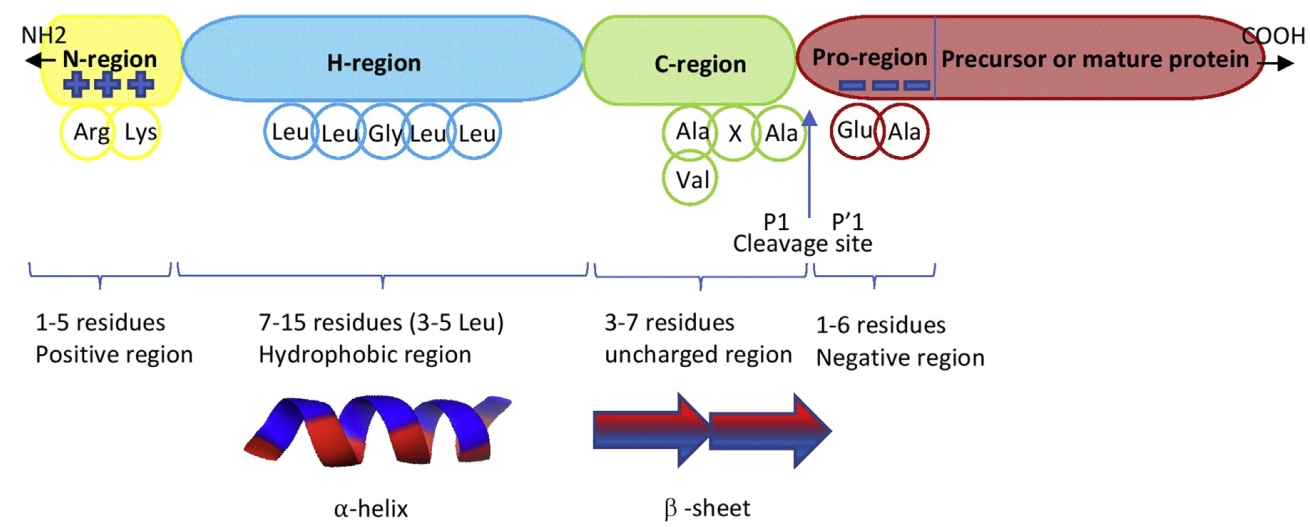
\includegraphics[width=\linewidth]
{./literature_review/subcellular_location/signal_peptides/img/signal_peptide_structure.png}
	~\end{subfigure}
	\caption{~\textbf{The general structure of a signal peptide.}
		Three general regions are discriminated inside the signal peptide and one region in the mature protein:
		(i) At the N-terminal end, there is a positively charged region, or N-region.
		(ii) This is followed by the H-region, or hydrophobic core, which forms the $\alpha$-helix.
		(iii) The C-region (C-terminal end) is where the cleavage site is situated,
		and forms a $\beta$-sheet.
		Residues before the cleavage site get a P notation,
		residues after it get a P' notation.
		The cleavage itself occurs after recognition of of the AXA or VXA motif.
		(iv) Downstream of the cleavage site, it he pro-region. 
		It is negatively charged and interacts with N-region to form a loop structure
		(from~\cite{owji2018}).}
	\label{fig:signal_peptide_structure}
~\end{figure}

